\documentclass[11pt,twoside]{article}
\usepackage{graphicx} % Required for inserting images
\usepackage[utf8]{inputenc}
\usepackage[T1]{fontenc}
\usepackage[french]{babel}
\usepackage{float}
\usepackage[
    left=3.18cm,
    right=3.18cm,
    top=2.54cm,
    bottom=2.54cm
]{geometry}
\usepackage{fancyhdr}

\pagestyle{fancy}

\fancyhf{} % clear all headers and footers

\fancyfoot[RO]{\thepage} % Right side on Odd pages
\fancyfoot[LE]{\thepage} % Left side on Even pages
\renewcommand{\headrulewidth}{0pt}
\renewcommand{\footrulewidth}{0pt}

\usepackage{setspace}
\setstretch{1.15}

\usepackage{amsmath} % for \numberwithin
\numberwithin{figure}{section}

\usepackage{caption}
\captionsetup{labelsep=colon,labelfont={footnotesize,bf},textfont={footnotesize,normalfont}}

\begin{document}

\begin{titlepage}
\centering

\vspace*{1cm}

{\Large \textbf{Caractérisation de thermocouples}} \\[0.5cm]
{\large Rapport des travaux pratiques 6 et 7, cours GMC-3006} \\[0.5cm]


\vfill

Travail présenté à Mme Janika Bourgeois et M. André Chamberland \\ [0.25cm]
Rédigé par \textbf{Zied Gharbi (536961413)} et \textbf{Charles Bouthilier (536842818)}

\vfill

Faculté des sciences et de génie \\ [0.25cm]
Génie mécanique \\ [0.25cm]
Université Laval

\vspace{0.5cm}

27 mars 2026

\end{titlepage}

\tableofcontents
\newpage


%Introduction
\newpage
\thispagestyle{empty}
\section{Introduction}

% Partie 1
\newpage
\section{Étalonnage dynamique de thermocouples (TP 6)}
\thispagestyle{empty}
\subsection{But}
L'objectif de la partie 1 du TP6 est de déterminer la constante de temps pour des thermocouples de différents diamètres, puis comparer les résultats obtenus.
\subsection{Graphiques}

%Graph 1
\setcounter{section}{1}
\begin{figure} [H]
    \centering
    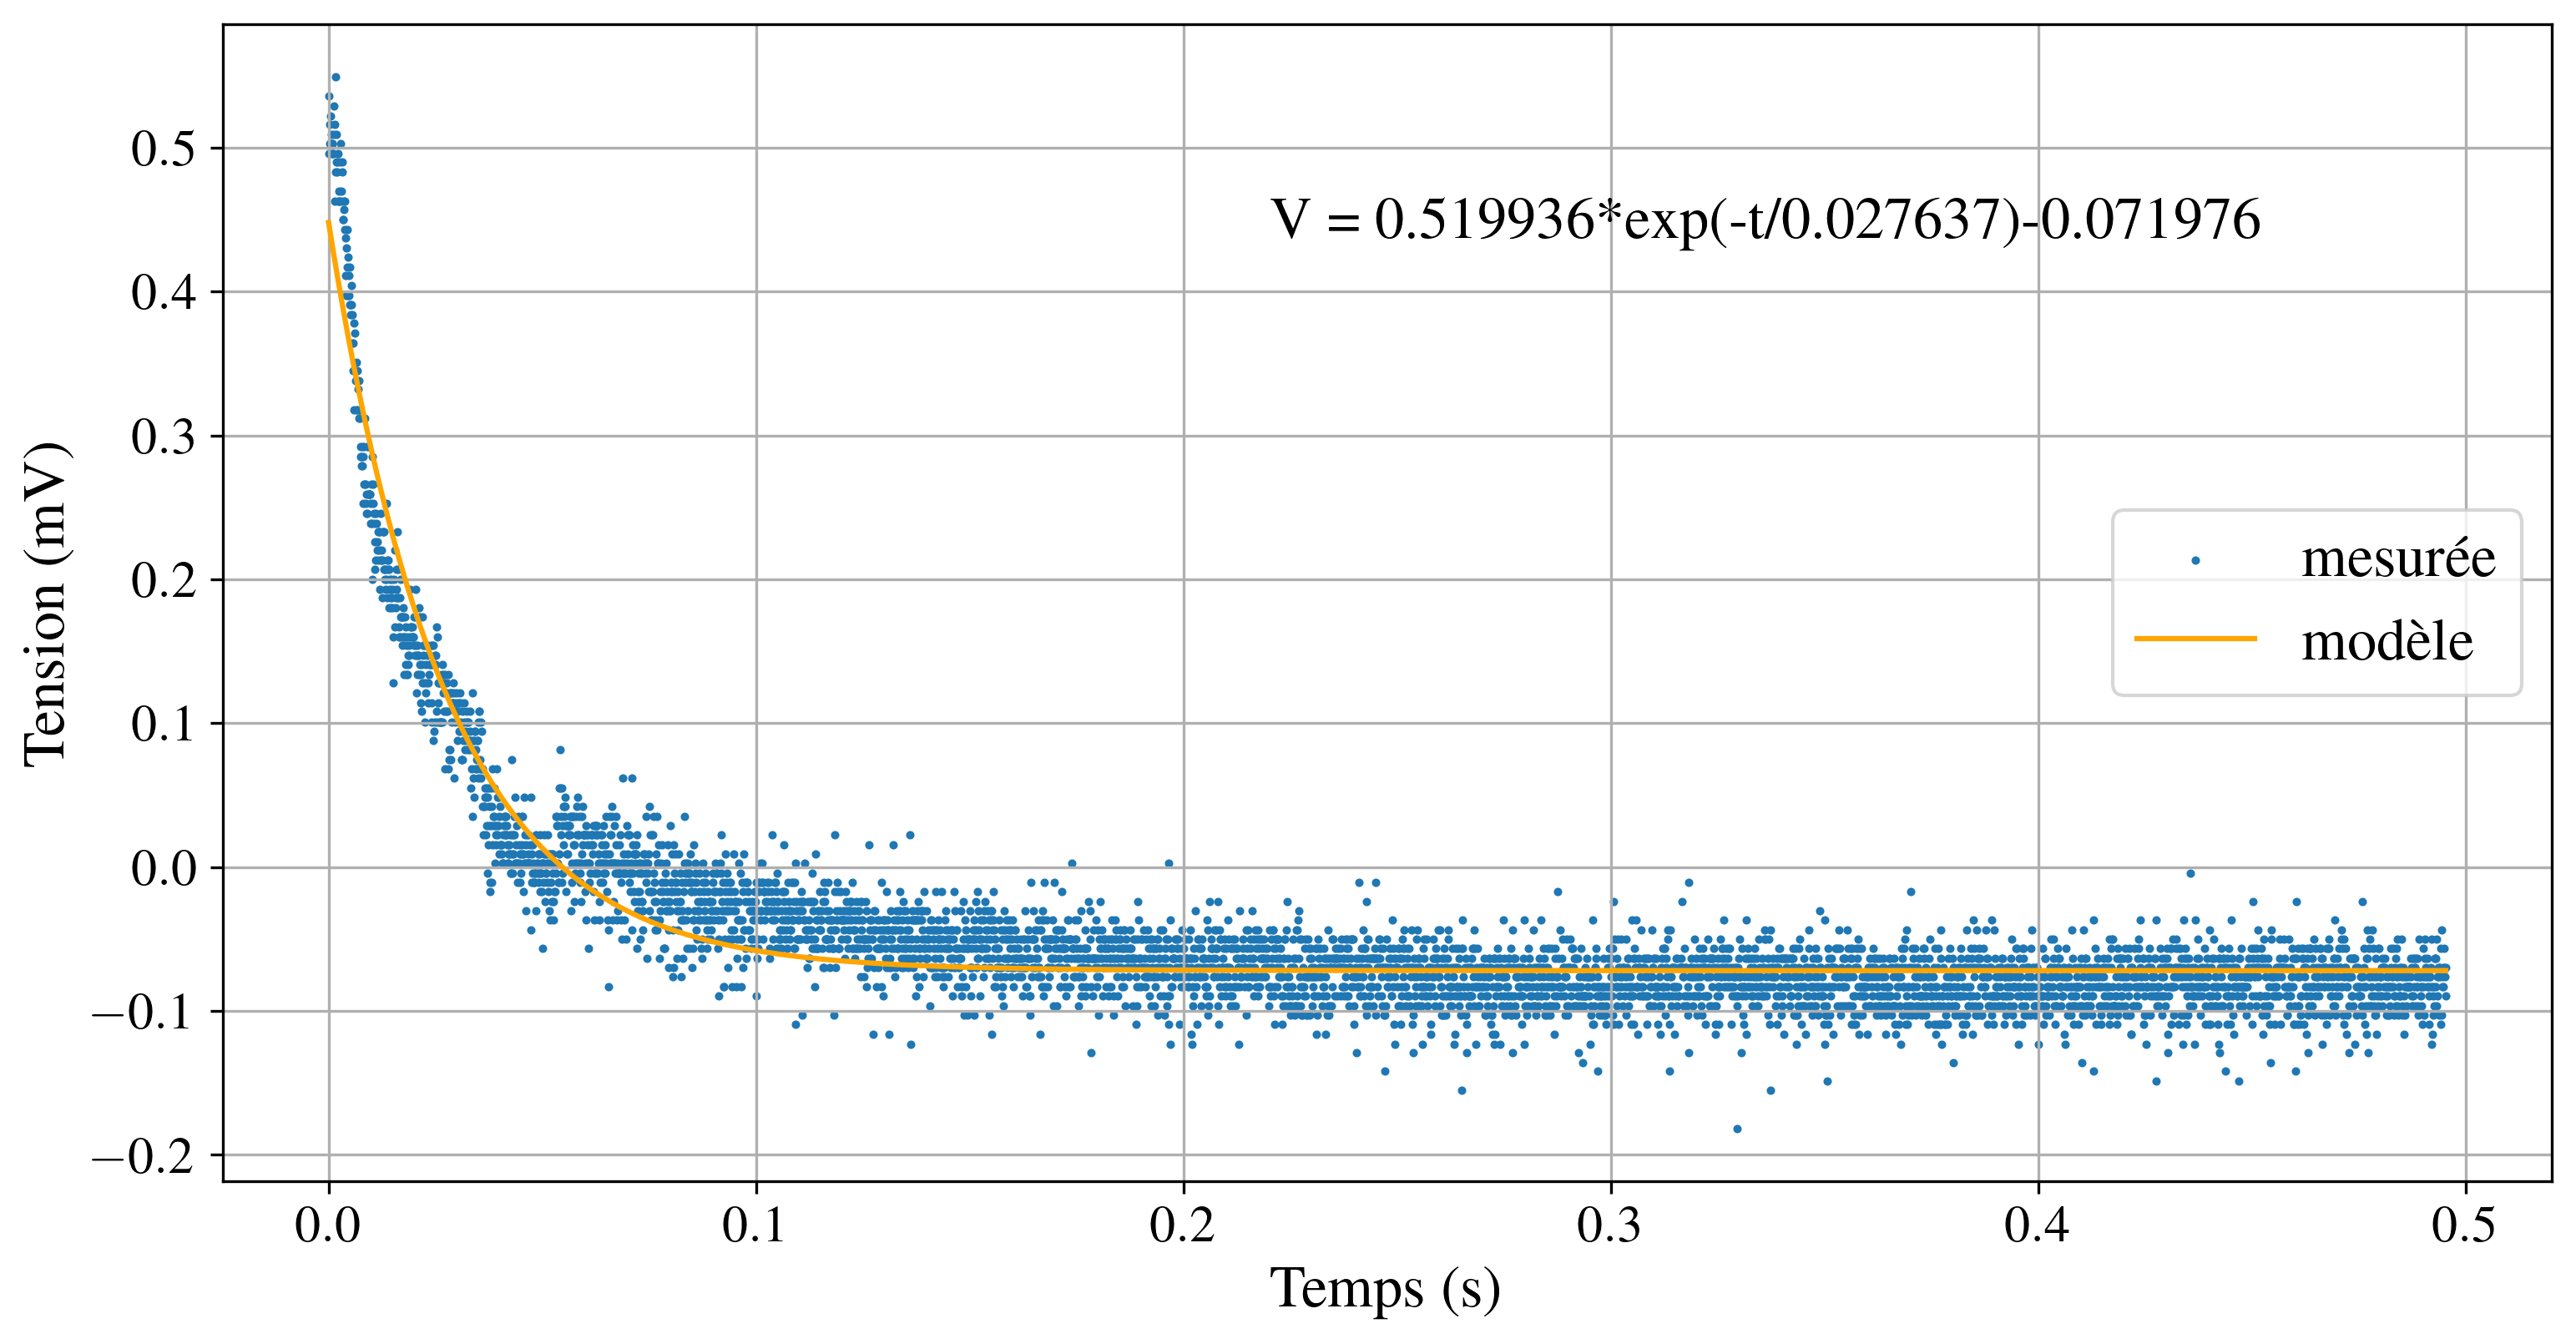
\includegraphics[width=1\linewidth]{graphs/TC_0005_s_filtre_50mvno_title.png}
    \caption{Tension mesurée au bornes d’un thermocouple de 0.005 po de diamètre lorsque plongé dans un bain d'eau glacée depuis une pièce à 23.9°C, acquise sur une gamme de -50 à 50 mV pendant trois secondes à une fréquence de 10 kHz, ainsi que la courbe de tendance modèlisée à partir des donnés. Les donnés ont été recadrées pour pour exclure le temps d'acquisition antérieur à la plongée afin d'ameliorer la qualité du modèle exponentiel. Les points ne sont pas liés entre eux pour apprécié l'effet de la fréquence et la gamme d'acquisition sur la prise de mesures}
    \label{fig:placeholder}
\end{figure}

%Graph 2
\begin{figure} [H]
    \centering
    
\includegraphics[width=1\linewidth]{graphs/TC_010_s_filtreno_title.png}
    \caption{Tension mesurée au bornes d’un thermocouple de 0.010 po de diamètre lorsque plongé dans un bain d'eau glacée depuis une pièce à 23.9°C, acquise sur une gamme de -50 à 50 mV pendant trois secondes à une fréquence de 10 kHz, ainsi que la courbe de tendance modèlisée à partir des donnés.}
    \label{fig:placeholder}
\end{figure}

%Graph 3
\begin{figure}
    \centering
    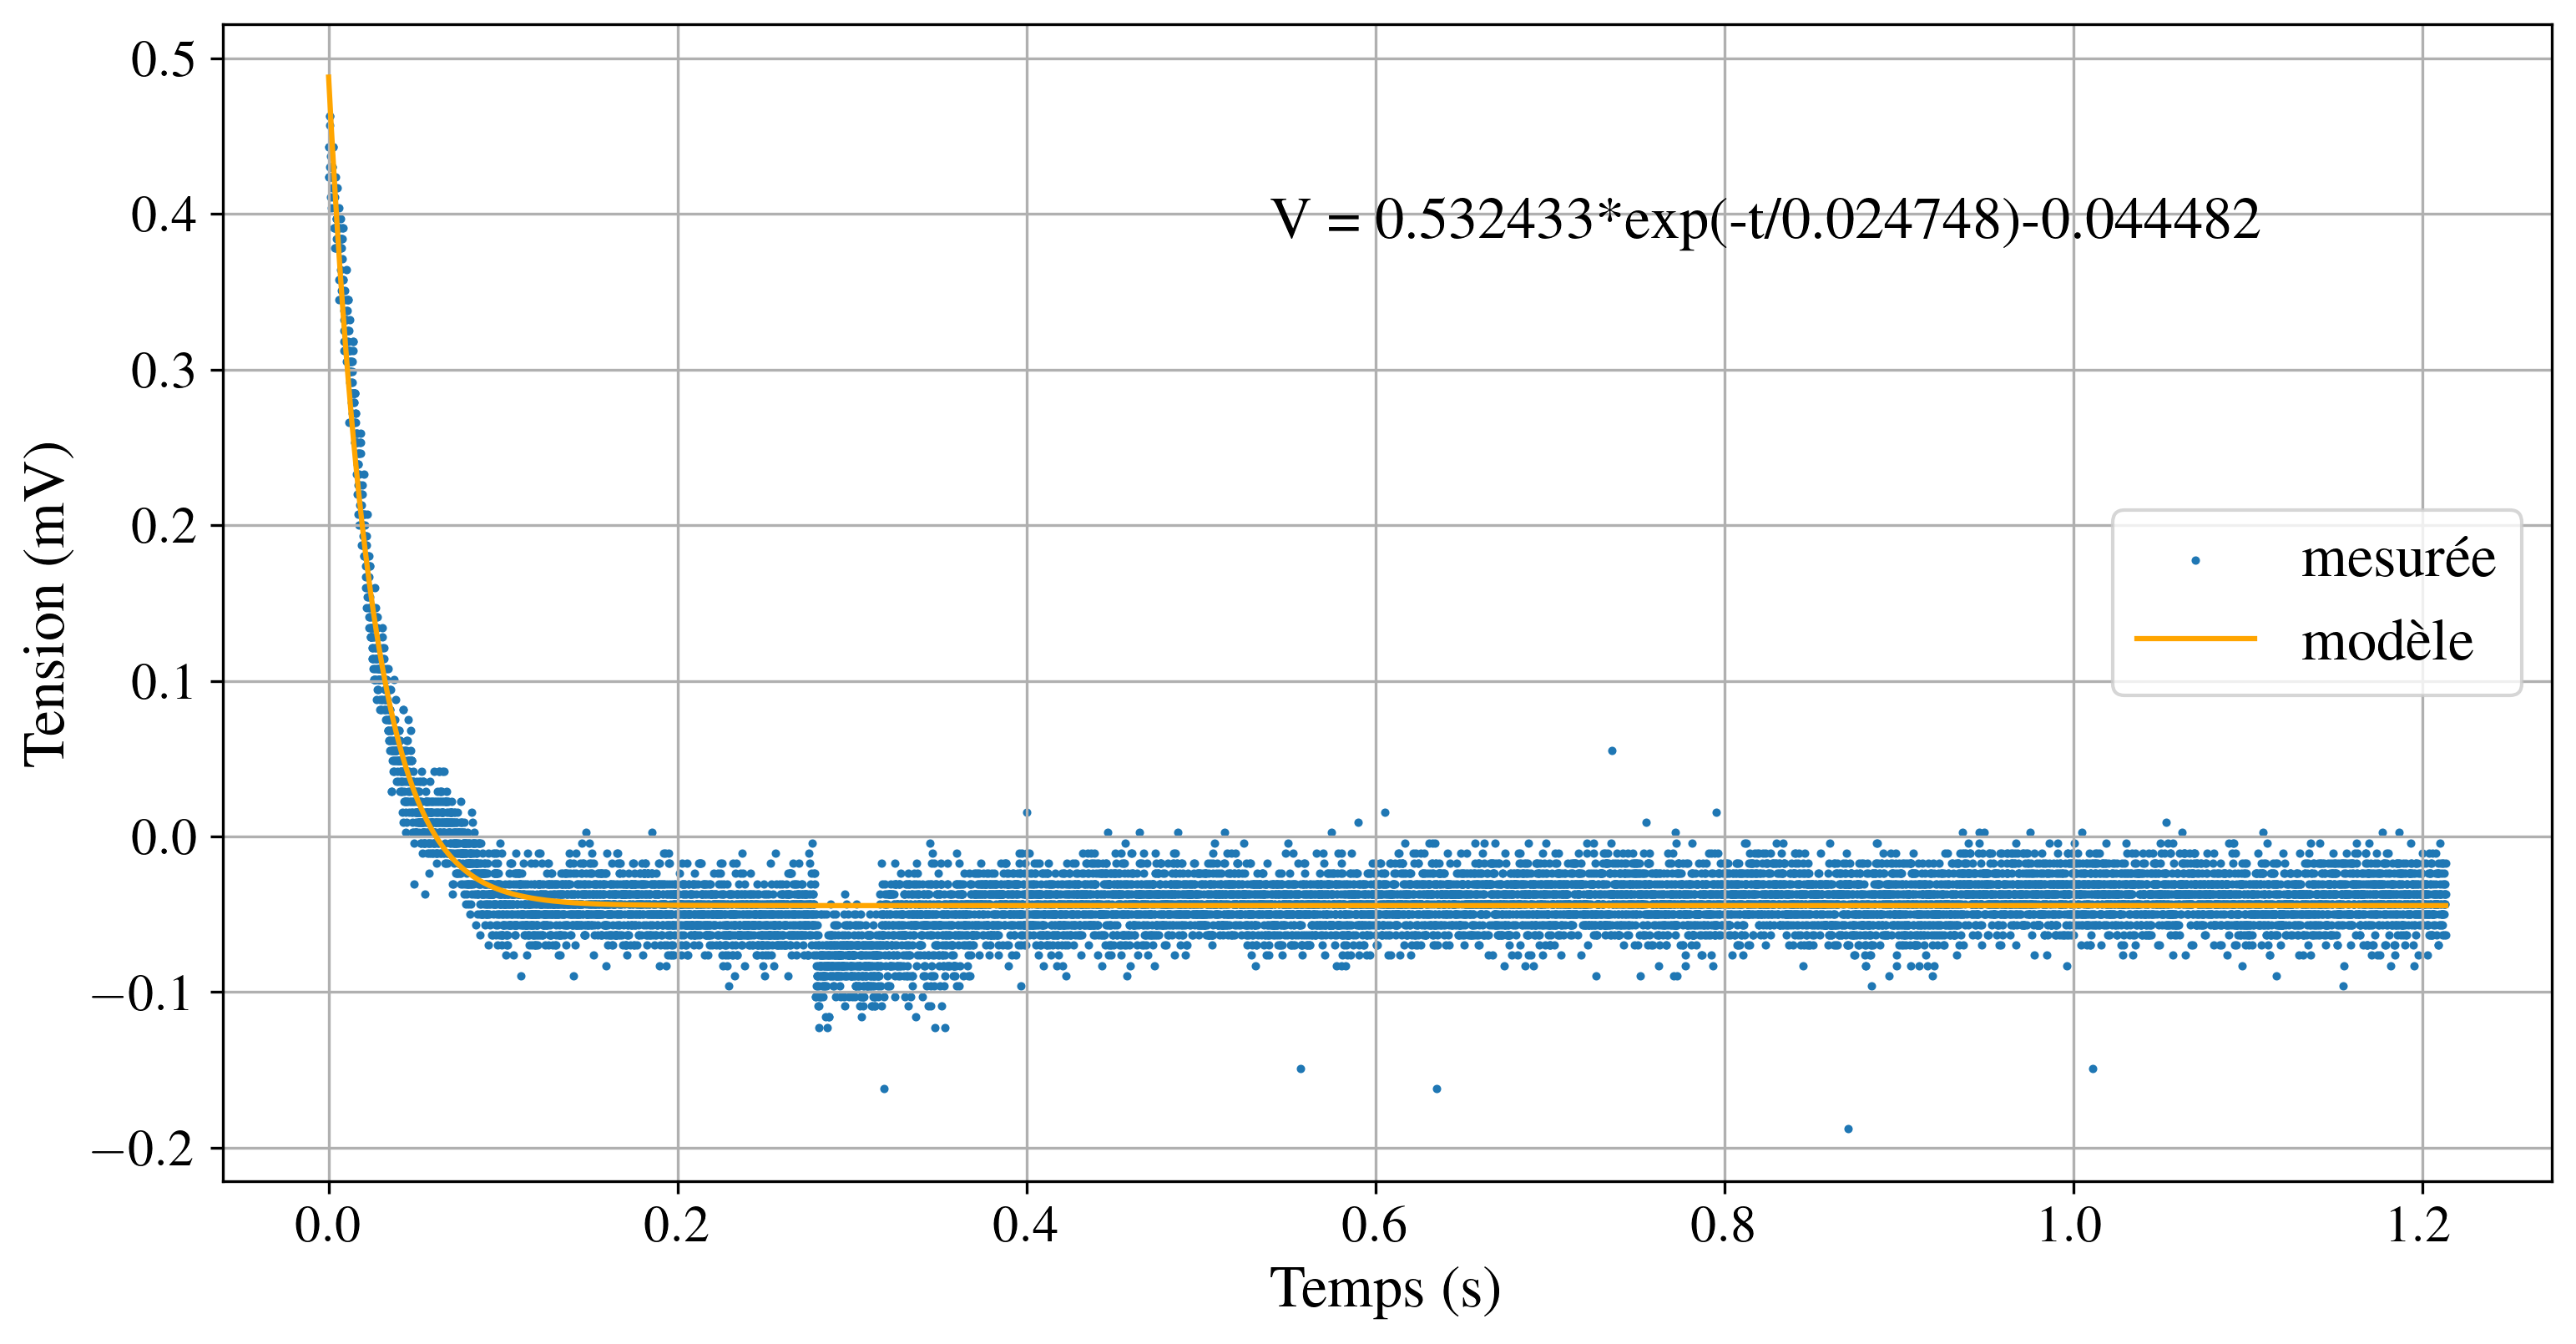
\includegraphics[width=1\linewidth]{graphs/TC_0020_s_filtreno_title.png}
    \caption{Tension mesurée au bornes d’un thermocouple de 0.020 po de diamètre lorsque plongé dans un bain d'eau glacée depuis une pièce à 23.9°C, acquise sur une gamme de -50 à 50 mV pendant trois secondes à une fréquence de 10 kHz, ainsi que la courbe de tendance modèlisée à partir des donnés.}
    \label{fig:placeholder}
\end{figure}

%Graph 4
\begin{figure}
    \centering
    
\includegraphics[width=1\linewidth]{graphs/TC_0032_s_filtreno_title.png}
    \caption{Tension mesurée au bornes d’un thermocouple de 0.032 po de diamètre lorsque plongé dans un bain d'eau glacée depuis une pièce à 23.9°C, acquise sur une gamme de -50 à 50 mV pendant trois secondes à une fréquence de 10 kHz, ainsi que la courbe de tendance modèlisée à partir des donnés.}
    \label{fig:placeholder}
\end{figure}

%Graph 5
\begin{figure}
    \centering
    
\includegraphics[width=1\linewidth]{graphs/TC_0005_s_filtre_10v_2no_title.png}
    \caption{Tension mesurée au bornes d’un thermocouple de 0.005 po de diamètre lorsque plongé dans un bain d'eau glacée depuis une pièce à 23.9°C, acquise sur une gamme de -10 à 10 V pendant trois secondes à une fréquence de 10 kHz, ainsi que la courbe de tendance modèlisée à partir des donnés.}    \label{fig:placeholder}
\end{figure}
\setcounter{section}{2}
\subsection{Tableau}
%Tableau tau des thermocouples
\begin{table}[H]
    \centering
    \caption{Constantes de temps des différents thermocouple}
    \label{tab:placeholder_label}
    \begin{tabular}{|c|c|c|}
        \hline
        Diamètre thermocouple [po] & Gamme de prise de mesure & Constante de temps [s] \\
        \hline
        0.005 & [-10;10] V  & 1.005362 \\
        \hline
        0.005  & [-50;50] mV & 0.027637 \\
        \hline
        0.01  & [-50;50] mV & 0.083208 \\
        \hline
        0.02  & [-50;50] mV & 0.024748 \\
        \hline
        0.032 & [-50;50] mV & 0.063595 \\
        \hline
    \end{tabular}
\end{table}

\subsection{Discussion}
La constante de temps la plus faible observée est de 0,024748 s, associée au thermocouple de 0,02 pouces de diamètre. Ainsi, ce thermocouple serait le plus réactif, c’est-à-dire celui qui répond le plus rapidement aux variations de température.

Cette observation constitue toutefois une contradiction avec le résultat attendu. En effet, selon la théorie, le thermocouple ayant le plus petit diamètre devrait posséder la constante de temps la plus faible. Plus précisément, la constante de temps dépend de la masse du thermocouple ainsi que de son efficacité à transférer la chaleur. Par conséquent, un thermocouple de plus petit diamètre possède une masse plus faible, ce qui devrait se traduire par une constante de temps plus faible.\cite{huang2024thermocouple} Cependant, les résultats observés indiquent que le plus petit thermocouple de 0,005 po possède une constante de temps de 0,027637 s, qui est supérieure à la constante de temps associée au thermocouple de 0,02 po.

La figure 5 représente l'essai effectué pour une gamme de -10 à 10 V. Les points de ce graphique ne suivent pas une tendance linéaire, et il n'est donc pas possible d'obtenir une courbe de régression valide. Ce phénomène est causé par la gamme d'acquisition trop élevée, qui dépasse l'amplitude normale du signal du thermocouple (de l'ordre de quelques millivolts).\cite{electronicdesign} Le signal est ainsi saturé et fortement bruité, ce qui produit des résultats inexacts. Par conséquent, la courbe de régression linéaire obtenue n'est pas représentative de la relation entre la tension du thermocouple et le temps. La gamme utilisée est donc trop élevée par rapport aux signaux réellement captés par le thermocouple.

%Partie 2
\newpage{}
\section{Fabrication d’un thermocouple (TP 6)}
\thispagestyle{empty}

\subsection{But}
L’objectif de la partie 2 du TP6 est de comprendre le fonctionnement et la fabrication d’un thermocouple. Cette partie inclut également la vérification et l’évaluation de l’efficacité du thermocouple fabriqué.

\subsection{Tableau}
% Requires: \usepackage{multirow}
\begin{table}[h]
    \centering
    \caption{Placeholder Caption}
    \label{tab:placeholder_label}
    \begin{tabular}{|l|c|c|}
        \hline
        & \multicolumn{2}{c|}{Température en fonction du milieu [\(^\circ\)C]} \\ \cline{2-3}
        & Air ambient & Eau chaude \\ \hline
        Thermomètre électronique & 23.9 & 47.0 \\ \hline
        Thermocouple, sonde de référence dans l'eau glacée & 20.3 & 42.4 \\ \hline
        Thermocouple, module de compensation & 25.9 & 44.3 \\ \hline
        Thermomètre à l'alcool & 23.5 & 48.0 \\ \hline
    \end{tabular}
\end{table}

\subsection{Discussion}
\textbf{Comparaison des résultats pour la température ambiante:} \\
Tout d’abord, les résultats du thermomètre électrique et du thermomètre à alcool présentent des températures similaires pour l’air ambiant. Ces mesures suggèrent que la température ambiante réelle serait d’environ 24 °C. Le résultat obtenu par le thermocouple avec la sonde dans l’eau glacée est inférieur aux résultats obtenus avec les thermomètres. Alors que le résultat obtenu avec le thermocouple utilisant le module de compensation est supérieur aux résultats obtenus avec les thermomètres. Cependant, les résultats restent dans le même ordre de grandeur avec un écart de quelques degrés. \\
Plusieurs sources d'erreurs peuvent expliquer la différence entre les résultats obtenus. Notamment, une mauvaise calibration du module de compensation pourrait être la cause de la température obtenue, qui est supérieure à celle attendue. La valeur de température inférieure obtenue par le thermocouple avec la sonde de référence dans l'eau glacée pourrait venir de l’aspect instable de la température de l'eau pour la sonde. De plus, une imperfection lors de la fabrication du thermocouple pourrait aussi expliquer les différents résultats obtenus pour la température. \\

\textbf{Comparaison des résultats pour la température de l'eau chaude:} \\
Tout d’abord, les résultats du thermomètre électrique et du thermomètre à alcool présentent des températures similaires pour l’eau chaude. Ces mesures suggèrent que la température de l’eau chaude serait située entre 47 °C et 48 °C. Les mesures avec les thermocouples sont plus basses que celles obtenues avec les thermomètres. Plus précisément, les résultats des thermocouples suggèrent une température de l’eau chaude autour de 43 °C, ce qui représente 4 à 5 °C de différence avec les mesures obtenues avec les thermomètres.\\ 
Plusieurs sources d'erreurs peuvent expliquer la différence entre les résultats de température. Entre autres, l'instabilité de la température de l'eau chaude, qui diminuait avec le temps, pourrait expliquer une partie de cet écart. Ainsi, une imperfection au sein du thermocouple pourrait également expliquer les résultats de températures inférieures obtenus par le thermocouple.

%Partie 3
\newpage{}
\section{Étalonnage statique de Thermocouples (TP 7)}
\thispagestyle{empty}
\subsection{But}
\subsection{Graphiques}
\subsection{Tableau}
\subsection{Discussion}

%Conclusion
\newpage
\thispagestyle{empty}
\section{Conclusion}

%Bibliographie
\newpage
\thispagestyle{empty}
\begin{thebibliography}{9}

\bibitem{huang2024thermocouple}
Huang, Qinghuang; Yue, Lingling; Li, Xingyou; Wang, Peiyong, 
"A correlation to calculate time constant of thermocouples," 
\textit{Applied Thermal Engineering}, vol. 246, 2024.  \texttt{https://www.sciencedirect.com/science/article/abs/pii/S135943112400588X}

\bibitem{electronicdesign}
“Key DAQ Specifications,” Electronic Design, 
\texttt{https://www.electronicdesign.com/home/article/21201396/key-daq-specifications}


\end{thebibliography}

\end{document}
